\documentclass[a4paper,12pt]{article}
\usepackage[utf8]{vietnam}
\usepackage[utf8]{inputenc}
\usepackage[T5]{fontenc}
\usepackage[margin=2.5cm]{geometry}
\usepackage{graphicx}
\usepackage{tikz}
\usepackage{fancyhdr}
\usepackage{float}
\usepackage[colorlinks=true, linkcolor=black, urlcolor=blue, citecolor=blue]{hyperref}
\usepackage{amsmath}
\usepackage{setspace}
\usepackage{xcolor}
\usepackage{booktabs}
\graphicspath{{./}}

\pagestyle{fancy}
\fancyhf{}
\renewcommand{\headrulewidth}{0pt}
\renewcommand{\footrulewidth}{0pt}
\fancyfoot[C]{\thepage}

\definecolor{lightblue}{rgb}{0.68, 0.85, 0.90}
\setstretch{1.2}
\setlength{\parindent}{0pt}
\setlength{\parskip}{0.4em}
\newcommand{\bai}[1]{\clearpage\setcounter{section}{0}\setcounter{equation}{0}\addcontentsline{toc}{part}{#1}{\LARGE\bfseries #1}\par\vspace{0.8em}}

\begin{document}
\begin{titlepage}
\begin{tikzpicture}[remember picture,overlay,inner sep=0,outer sep=0]
     \draw[blue!70!black,line width=4pt] ([xshift=-1.5cm,yshift=-2cm]current page.north east) coordinate (A)--([xshift=1.5cm,yshift=-2cm]current page.north west) coordinate(B)--([xshift=1.5cm,yshift=2cm]current page.south west) coordinate (C)--([xshift=-1.5cm,yshift=2cm]current page.south east) coordinate(D)--cycle;

     \draw ([yshift=0.5cm,xshift=-0.5cm]A)-- ([yshift=0.5cm,xshift=0.5cm]B)--
     ([yshift=-0.5cm,xshift=0.5cm]B) --([yshift=-0.5cm,xshift=-0.5cm]B)--([yshift=0.5cm,xshift=-0.5cm]C)--([yshift=0.5cm,xshift=0.5cm]C)--([yshift=-0.5cm,xshift=0.5cm]C)-- ([yshift=-0.5cm,xshift=-0.5cm]D)--([yshift=0.5cm,xshift=-0.5cm]D)--([yshift=0.5cm,xshift=0.5cm]D)--([yshift=-0.5cm,xshift=0.5cm]A)--([yshift=-0.5cm,xshift=-0.5cm]A)--([yshift=0.5cm,xshift=-0.5cm]A);


     \draw ([yshift=-0.3cm,xshift=0.3cm]A)-- ([yshift=-0.3cm,xshift=-0.3cm]B)--
     ([yshift=0.3cm,xshift=-0.3cm]B) --([yshift=0.3cm,xshift=0.3cm]B)--([yshift=-0.3cm,xshift=0.3cm]C)--([yshift=-0.3cm,xshift=-0.3cm]C)--([yshift=0.3cm,xshift=-0.3cm]C)-- ([yshift=0.3cm,xshift=0.3cm]D)--([yshift=-0.3cm,xshift=0.3cm]D)--([yshift=-0.3cm,xshift=-0.3cm]D)--([yshift=0.3cm,xshift=-0.3cm]A)--([yshift=0.3cm,xshift=0.3cm]A)--([yshift=-0.3cm,xshift=0.3cm]A);

\end{tikzpicture}

\begin{center}
    \vspace{0.5cm}
    {\bf\Large ĐẠI HỌC QUỐC GIA HÀ NỘI}\\[0.5em]
    {\bf\Large TRƯỜNG ĐẠI HỌC CÔNG NGHỆ}\\[2em]

    \vspace{8pt}
    
\includegraphics[width=0.35\textwidth]{logo.png}\\[2em]
    \vspace{8pt}

    {\bf\LARGE BÁO CÁO THỰC HÀNH 4 \\[0.5em]
    \bf\LARGE XỬ LÝ ẢNH VÀ THỊ GIÁC ROBOT}\\[6em]
\end{center}

\begin{flushleft}

    \hspace*{3.2cm} {\bf\LARGE Giảng viên hướng dẫn:  }\\[0.7em]
    \hspace*{3.2cm} {\LARGE Bùi Đình Đăng }\\[3em]

    \hspace*{3.2cm} {\bf\LARGE Sinh viên thực hiện: }\\[0.7em]
    \hspace*{3.2cm} {\LARGE Lương Nguyễn Việt Sang - 23020762}\\[0.9em]
\end{flushleft}

\end{titlepage}

\tableofcontents
\newpage

%================ BÀI 1 ================
\bai{Bài 1 - Xây dựng phép biến đổi DFT và IDFT}

\section{Đề bài}
Tự cài đặt DFT và IDFT hai chiều (không dùng \texttt{np.fft}), tính và hiển thị phần thực, phần ảo, phổ biên độ, pha, thực hiện dịch tâm phổ không dùng \texttt{fftshift}, khôi phục ảnh bằng IDFT, giải thích vì sao phổ được hiển thị dưới dạng $\log(1+|F|)$ và nhận xét sai số khôi phục. Áp dụng với \texttt{lena.png} thu nhỏ về $64\times 64$.

\section{Cơ sở lý thuyết}
Với ảnh $f(x,y)$ kích thước $M\times N$:
\begin{equation}
F(u,v)=\sum_{x=0}^{M-1}\sum_{y=0}^{N-1} f(x,y)\,e^{-j2\pi\left(\frac{ux}{M}+\frac{vy}{N}\right)},\quad
f(x,y)=\frac{1}{MN}\sum_{u=0}^{M-1}\sum_{v=0}^{N-1} F(u,v)\,e^{j2\pi\left(\frac{ux}{M}+\frac{vy}{N}\right)}.
\end{equation}
Hạt nhân tách được theo $x$ và $y$ nên tổng kép viết được thành $\mathbf{F}=\mathbf{W}_M\,\mathbf{f}\,\mathbf{W}_N$ với $W_n[k,m]=e^{-j2\pi km/n}$. IDFT dùng ma trận liên hợp và chia cho $MN$. Phổ biên độ và pha là
\begin{equation}
|F|=\sqrt{R^2+I^2},\qquad \phi=\operatorname{atan2}(I,R).
\end{equation}
Thành phần tần số 0 nằm ở góc ma trận $F$, nên ta dịch vòng hàng và cột đi $M/2$, $N/2$ (hoán vị chỉ số) để đưa nó về giữa phổ. Do dải động của $|F|$ rất lớn, phổ được hiển thị dưới dạng
\begin{equation}
S(u,v)=\log\big(1+|F(u,v)|\big),
\end{equation}
và sai số khôi phục được đo bằng $\mathrm{MSE}=\frac{1}{MN}\sum_{x,y}[f(x,y)-\hat f(x,y)]^2$.

\section{Kết quả thực nghiệm và phân tích}
\begin{figure}[H]
    \centering
    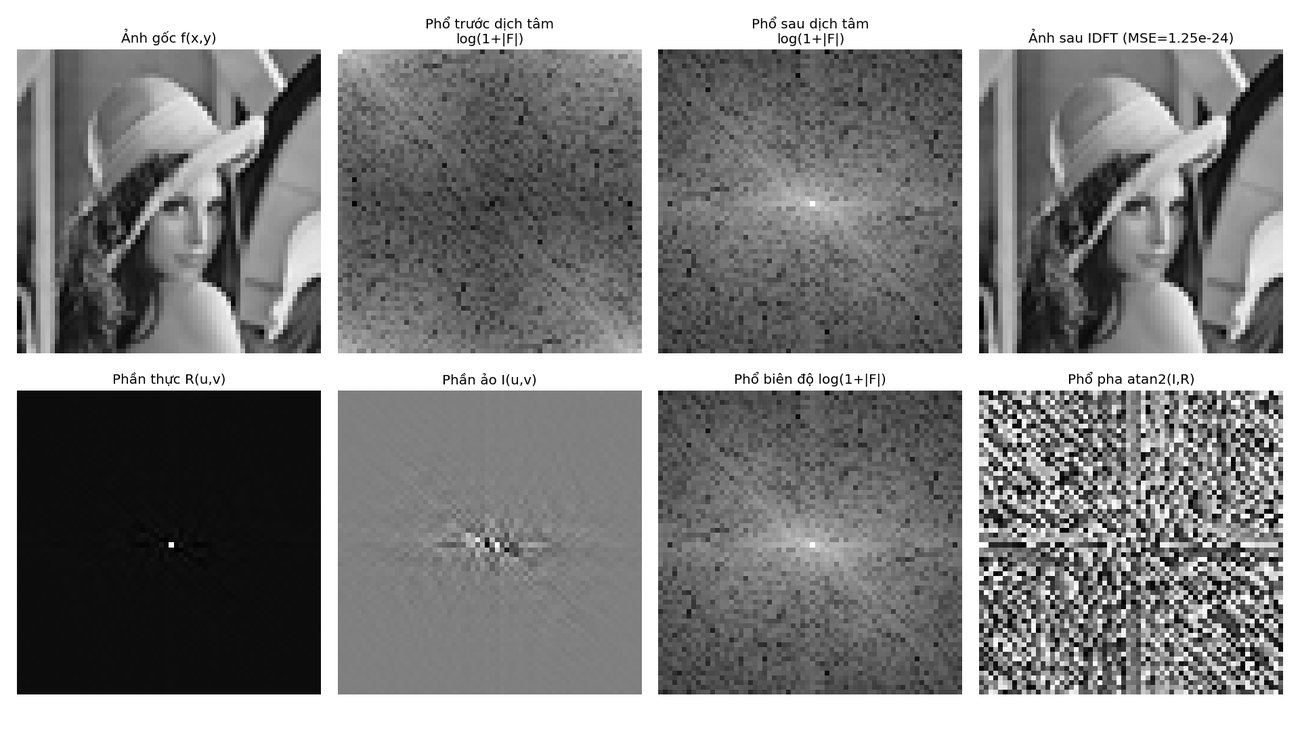
\includegraphics[width=\textwidth]{bai1_result.jpg}
    \caption{Hàng trên: ảnh gốc, phổ trước dịch tâm, phổ sau dịch tâm, ảnh sau IDFT. Hàng dưới: phần thực, phần ảo, phổ biên độ, phổ pha (đã dịch tâm)}
\end{figure}

\begin{table}[H]
\centering
\begin{tabular}{lr}
\toprule
Đại lượng & Giá trị \\
\midrule
$|F(0,0)|$ (thành phần DC) & $508\,066$ \\
$\max|F|$ không tính DC & $38\,053$ \\
Trung vị của $|F|$ & $628$ \\
MSE giữa ảnh gốc và ảnh sau IDFT & $1{,}25\times 10^{-24}$ \\
MSE sau khi làm tròn về 8 bit & $0$ \\
\bottomrule
\end{tabular}
\caption{Thống kê phổ và sai số khôi phục}
\end{table}

\textbf{Nhận xét:}
\begin{itemize}
    \item Sau khi dịch tâm, các tần số thấp từ bốn góc gom về giữa phổ, điểm sáng nhất là thành phần DC. Phổ có dạng chữ thập sáng, rõ hơn theo phương ngang, do các cạnh ngang và dọc mạnh trong ảnh và do DFT coi ảnh là tuần hoàn.
    \item Thành phần DC lớn gấp khoảng $13$ lần hệ số lớn nhất còn lại và hơn $800$ lần trung vị. Nếu hiển thị tuyến tính thì chỉ thấy một điểm sáng, còn thang log nén dải động để thấy được cấu trúc các tần số còn lại. Số $1$ tránh $\log 0$.
    \item Phổ pha trông như nhiễu nhưng mang thông tin về vị trí và hình dạng cạnh trong ảnh.
    \item MSE chỉ cỡ $10^{-24}$: DFT và IDFT là cặp biến đổi thuận nghịch chính xác, sai số còn lại chỉ là sai số làm tròn số dấu phẩy động, và sau khi làm tròn về 8 bit thì MSE bằng $0$.
\end{itemize}

%================ BÀI 2 ================
\bai{Bài 2 - DCT/IDCT cho khối ảnh $8\times 8$}

\section{Đề bài}
Tự cài đặt DCT và IDCT hai chiều cho khối ảnh $8\times 8$ lấy từ \texttt{lena.png}, hiển thị khối gốc, ma trận hệ số, hệ số DC, một số hệ số AC và khối sau IDCT, lưu ma trận hệ số vào tệp \texttt{.txt}, rồi đặt $50\%$, $75\%$, $90\%$ hệ số nhỏ nhất về $0$ và so sánh. Trả lời câu hỏi về ý nghĩa của $C(0,0)$ và các hệ số $C(u,v)$ với $(u,v)\neq(0,0)$.

\section{Cơ sở lý thuyết}
Với khối $N\times N$ ($N=8$):
\begin{equation}
C(u,v)=\alpha(u)\alpha(v)\sum_{x=0}^{N-1}\sum_{y=0}^{N-1} f(x,y)\cos\!\tfrac{(2x+1)u\pi}{2N}\cos\!\tfrac{(2y+1)v\pi}{2N},\quad
\alpha(k)=\begin{cases}\sqrt{1/N}, & k=0,\\ \sqrt{2/N}, & k>0.\end{cases}
\end{equation}
Đặt $A[u,x]=\alpha(u)\cos\frac{(2x+1)u\pi}{2N}$ thì $\mathbf{C}=A\mathbf{f}A^T$ và IDCT là $\mathbf{f}=A^T\mathbf{C}A$ vì $A$ trực giao. Hệ số $C(0,0)=N\bar f$ tỉ lệ với giá trị trung bình của khối, còn các hệ số AC mô tả sự biến thiên quanh giá trị đó, chỉ số càng lớn thì chi tiết càng mịn. Với $N=8$ thì $\alpha(0)=\frac{1}{2\sqrt2}$ và $\alpha(k)=\frac12$ với $k=1,\dots,7$. Chất lượng khối khôi phục được đo bằng MSE và $\mathrm{PSNR}=10\log_{10}(255^2/\mathrm{MSE})$.

\section{Kết quả thực nghiệm và phân tích}
Khối ảnh lấy tại hàng $240$, cột $240$ của \texttt{lena.png}.
\begin{figure}[H]
    \centering
    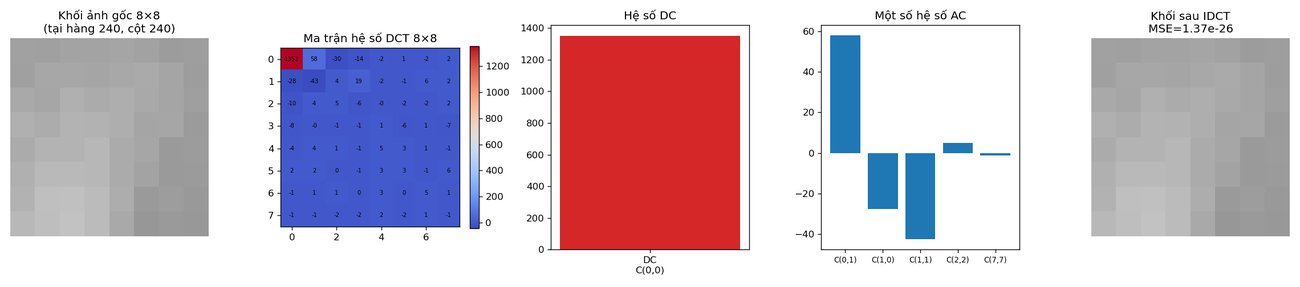
\includegraphics[width=\textwidth]{bai2_result.jpg}
    \caption{Khối gốc, ma trận hệ số DCT, hệ số DC, một số hệ số AC và khối sau IDCT}
\end{figure}
Ta có $C(0,0)=1352{,}375=8\times 169{,}05$, đúng bằng $8$ lần giá trị trung bình khối, trong khi các hệ số AC nhỏ hơn nhiều: $C(0,1)=58{,}12$, $C(1,0)=-27{,}70$, $C(1,1)=-42{,}54$, $C(7,7)=-1{,}09$. Khối sau IDCT trùng khối gốc với MSE cỡ $10^{-26}$. Ma trận hệ số được lưu trong \texttt{bai2\_dct\_coefficients.txt}.

\begin{figure}[H]
    \centering
    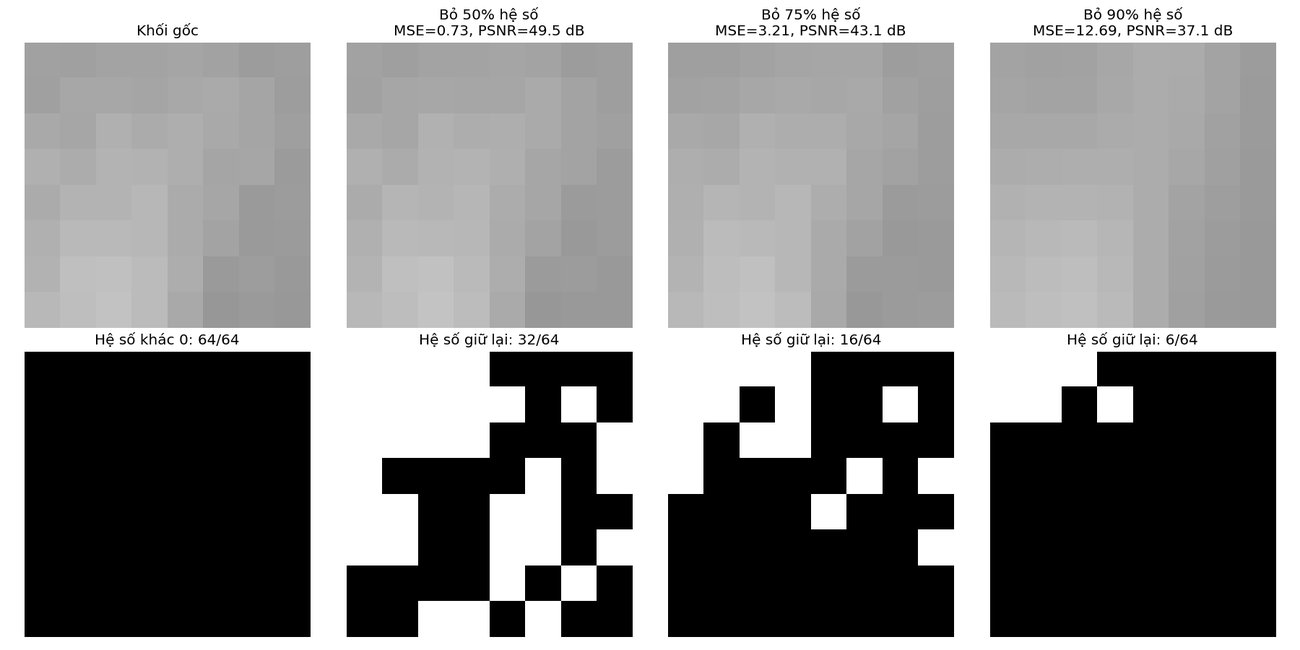
\includegraphics[width=0.9\textwidth]{bai2_loai_he_so.jpg}
    \caption{Khối ảnh sau khi bỏ $50\%$, $75\%$, $90\%$ hệ số nhỏ nhất (hàng trên) và các hệ số được giữ lại (hàng dưới)}
\end{figure}

\begin{table}[H]
\centering
\begin{tabular}{lccc}
\toprule
Tỉ lệ hệ số bị bỏ & Số hệ số giữ lại & MSE & PSNR (dB) \\
\midrule
$50\%$ & $32/64$ & $0{,}73$ & $49{,}52$ \\
$75\%$ & $16/64$ & $3{,}21$ & $43{,}06$ \\
$90\%$ & $6/64$ & $12{,}69$ & $37{,}10$ \\
\bottomrule
\end{tabular}
\caption{Chất lượng khối ảnh sau IDCT khi loại bỏ hệ số DCT nhỏ nhất}
\end{table}

\textbf{Nhận xét:}
\begin{itemize}
    \item Năng lượng tập trung ở hệ số DC và các hệ số tần số thấp ở góc trên bên trái, còn hệ số tần số cao gần $0$. Ảnh tự nhiên biến đổi chậm, các pixel lân cận tương quan mạnh nên phần lớn khối là vùng mịn.
    \item Bỏ $50\%$ hệ số hầu như không đổi ảnh (PSNR $49{,}5$ dB), bỏ $75\%$ vẫn đạt $43{,}1$ dB, và chỉ giữ $6$ hệ số vẫn còn $37{,}1$ dB, nhận ra được cấu trúc sáng tối nhưng chi tiết nhỏ bị làm mịn.
    \item Các hệ số AC nhỏ chủ yếu ứng với chi tiết mịn và nhiễu nên bỏ chúng chỉ gây sai số nhỏ. Đây là cơ sở của nén JPEG. Sai số tăng nhanh ở mức $90\%$ vì lúc đó đã bỏ cả các hệ số AC đáng kể như $C(1,1)$.
\end{itemize}

\subsection{Câu hỏi thảo luận}
Hệ số $C(0,0)$ mang thông tin gì? Hệ số $C(0,0)$ (hệ số DC) bằng $\frac{1}{8}\sum_{x,y}f(x,y)=8\bar f$, nên mang thông tin về độ sáng trung bình của khối. Ở khối thực nghiệm, $C(0,0)=1352{,}375$ tương ứng với giá trị trung bình $169{,}05$.

Vì sao năng lượng của ảnh tự nhiên thường tập trung ở vùng tần số thấp? Ảnh tự nhiên gồm chủ yếu các vùng mịn, trong đó cường độ các pixel lân cận gần bằng nhau, nên khối ảnh gần với một hàm biến đổi chậm. Các hàm cơ sở cosin tần số thấp biểu diễn tốt dạng này, còn thành phần tần số cao chỉ cần để biểu diễn những thay đổi nhanh (cạnh, kết cấu, nhiễu) vốn chiếm phần nhỏ. Vì vậy các hệ số lớn dồn vào góc trên bên trái ma trận, còn hệ số tần số cao gần $0$.

Các hệ số $C(u,v)$ với $(u,v)\neq(0,0)$ có vai trò gì? Đây là các hệ số AC, mỗi hệ số cho biết biên độ của một mẫu dao động cosin quanh giá trị trung bình, trong đó $u$ ứng với dao động theo chiều dọc, $v$ theo chiều ngang. Chỉ số càng lớn thì mẫu dao động càng mau, ứng với chi tiết mịn hơn. Chúng mang thông tin về cạnh và kết cấu, và việc bỏ các hệ số AC nhỏ chỉ làm mất chi tiết mịn mà không đổi độ sáng chung của khối.

%================ BÀI 3 ================
\bai{Bài 3 - Lọc thông thấp và thông cao lý tưởng}

\section{Đề bài}
Dùng DFT và IDFT ở Bài 1 để lọc ảnh trong miền tần số: tính khoảng cách tới tâm phổ, xây dựng bộ lọc thông thấp lý tưởng (ILPF) với $D_0=10,30,50$, lọc $G=HF$ rồi IDFT, xây dựng bộ lọc thông cao lý tưởng (IHPF), hiển thị ảnh gốc, phổ, mặt nạ và ảnh sau lọc. So sánh theo $D_0$ và giải thích vì sao bỏ tần số cao làm ảnh mờ, bỏ tần số thấp làm nổi bật cạnh. Áp dụng với \texttt{lena.png} thu nhỏ về $128\times 128$.

\section{Cơ sở lý thuyết}
Khoảng cách tới tâm phổ (đã dịch tâm) là $D(u,v)=\sqrt{(u-M/2)^2+(v-N/2)^2}$. Các bộ lọc là
\begin{equation}
H_{LP}(u,v)=\begin{cases}1, & D(u,v)\le D_0,\\ 0, & D(u,v)>D_0,\end{cases}\qquad H_{HP}=1-H_{LP},
\end{equation}
và phép lọc là $G(u,v)=H(u,v)F_s(u,v)$, sau đó đưa $G$ về thứ tự ban đầu và áp dụng IDFT, lấy phần thực.

\section{Kết quả thực nghiệm và phân tích}
\begin{figure}[H]
    \centering
    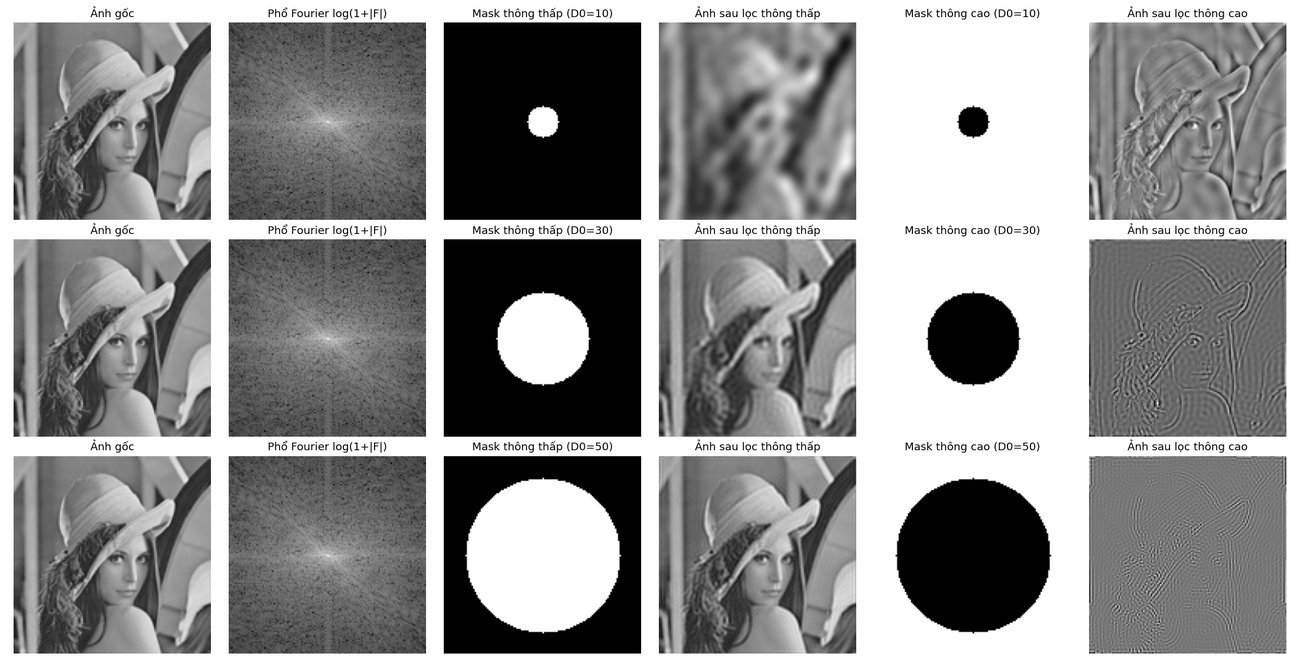
\includegraphics[width=\textwidth]{bai3_result.jpg}
    \caption{Lọc Ideal với $D_0=10,30,50$ (từng hàng): ảnh gốc, phổ, mặt nạ thông thấp, ảnh sau lọc thông thấp, mặt nạ thông cao, ảnh sau lọc thông cao}
\end{figure}

\begin{table}[H]
\centering
\begin{tabular}{ccc}
\toprule
$D_0$ & MSE (ảnh gốc, ảnh sau lọc) & Năng lượng phổ giữ lại \\
\midrule
$10$ & $514{,}82$ & $97{,}07\%$ \\
$30$ & $104{,}50$ & $99{,}41\%$ \\
$50$ & $24{,}54$ & $99{,}86\%$ \\
\bottomrule
\end{tabular}
\caption{Sai số của lọc thông thấp lý tưởng}
\end{table}

\textbf{Nhận xét:}
\begin{itemize}
    \item $D_0=10$ làm ảnh rất mờ và có vân sóng quanh vùng sáng tối. Khi $D_0$ tăng lên $30$ và $50$, ảnh rõ dần, MSE giảm từ $514{,}8$ xuống $104{,}5$ rồi $24{,}5$.
    \item Vòng tròn $D_0=10$ đã giữ $97{,}07\%$ năng lượng, cho thấy năng lượng tập trung ở tần số thấp, còn phần tần số cao tuy ít năng lượng nhưng quyết định độ sắc nét.
    \item Tần số cao ứng với thay đổi mức xám đột ngột (cạnh, kết cấu mịn, nhiễu), bỏ chúng làm chuyển tiếp mức xám thoải hơn nên ảnh mờ. Tần số thấp ứng với vùng phẳng và độ sáng nền, bỏ chúng thì vùng phẳng về xám trung tính và chỉ còn cạnh nổi bật.
    \item Mặt nạ cắt cứng $0/1$ gây ringing (vân sóng đồng tâm quanh cạnh).
\end{itemize}

\subsection{Yêu cầu đánh giá}
So sánh ảnh khi thay đổi $D_0$: $D_0$ càng nhỏ thì vùng thông càng hẹp, ảnh thông thấp càng mờ (MSE $514{,}8\to 104{,}5\to 24{,}5$ khi $D_0=10\to 30\to 50$) và ảnh thông cao càng giữ nhiều cấu trúc. $D_0$ càng lớn thì ảnh thông thấp càng giống ảnh gốc, còn ảnh thông cao chỉ còn các cạnh mảnh.

Vì sao loại bỏ tần số cao làm ảnh mờ, còn loại bỏ tần số thấp làm nổi bật cạnh? Tần số cao biểu diễn những thay đổi mức xám đột ngột nên chính chúng tạo ra độ sắc của cạnh và chi tiết. Khi loại bỏ chúng, chuyển tiếp mức xám trở nên thoải hơn và ảnh bị mờ. Tần số thấp biểu diễn vùng phẳng và độ sáng nền. Khi loại bỏ chúng, các vùng phẳng về mức xám trung tính và chỉ còn lại các biến thiên nhanh, tức là cạnh.

%================ BÀI 4 ================
\bai{Bài 4 - So sánh các bộ lọc Ideal, Gaussian và Butterworth}

\section{Đề bài}
Từ Bài 3, xây dựng ba bộ lọc thông thấp Ideal, Gaussian, Butterworth ($n=1,2,4$; $D_0=10,30,50,80$), hiển thị mặt nạ, phổ sau lọc và ảnh kết quả với cùng $D_0$, xây dựng bộ lọc thông cao tương ứng để làm sắc nét ảnh và so sánh chất lượng. Áp dụng với \texttt{lena.png} thu nhỏ về $128\times 128$.

\section{Cơ sở lý thuyết}
\begin{equation}
H_{G}=\exp\!\left(-\frac{D^2}{2D_0^2}\right),\qquad
H_{B}=\frac{1}{1+(D/D_0)^{2n}},\qquad H_{HP}=1-H_{LP}.
\end{equation}
Bộ lọc Gaussian suy giảm liên tục từ tâm ra ngoài. Bộ lọc Butterworth có độ dốc quanh $D_0$ do $n$ điều khiển: $n$ nhỏ cho chuyển tiếp êm, $n$ lớn tiến dần tới Ideal. Ảnh được làm sắc nét bằng $f_{\text{sharp}}=f+g_{HP}$, với $g_{HP}$ là ảnh thông cao.

\section{Kết quả thực nghiệm và phân tích}
\begin{figure}[H]
    \centering
    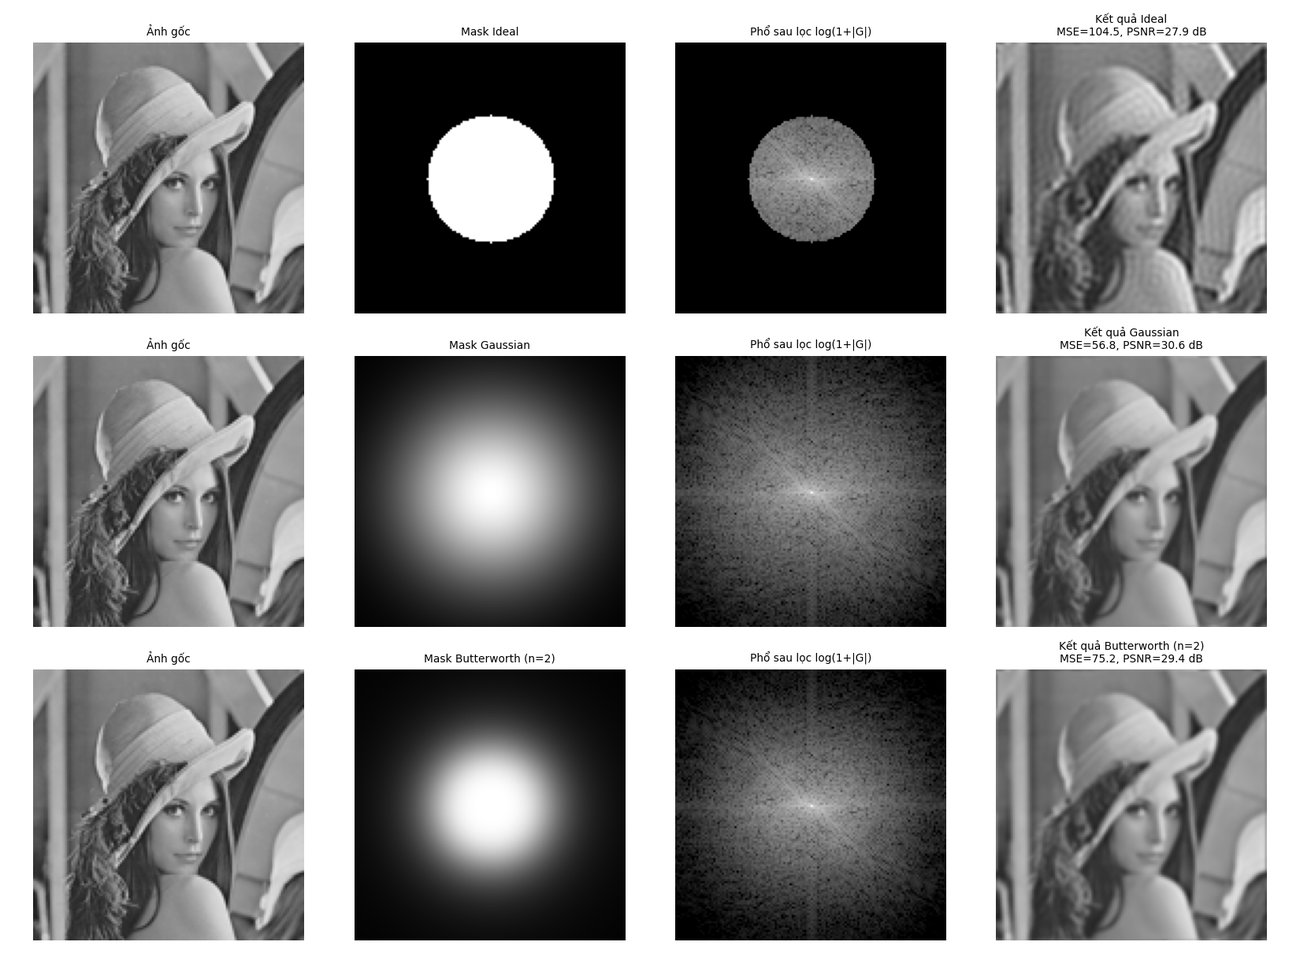
\includegraphics[width=0.9\textwidth]{bai4_so_sanh_D0_30.jpg}
    \caption{Mặt nạ, phổ sau lọc và ảnh kết quả của Ideal, Gaussian, Butterworth ($n=2$) với $D_0=30$}
\end{figure}

\begin{figure}[H]
    \centering
    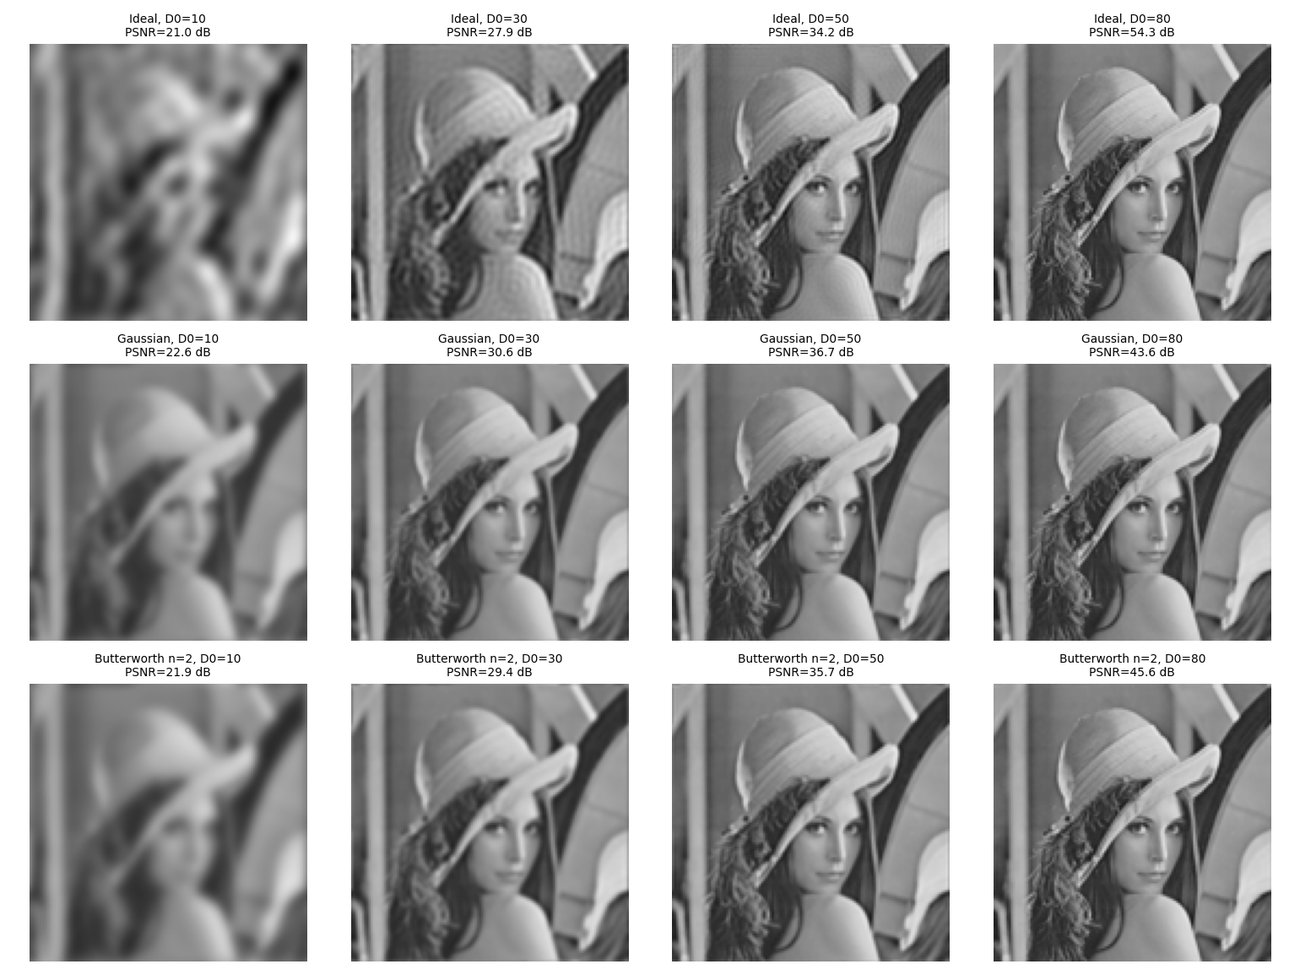
\includegraphics[width=0.9\textwidth]{bai4_D0.jpg}
    \caption{Ảnh sau lọc của Ideal, Gaussian, Butterworth ($n=2$) với $D_0=10,30,50,80$}
\end{figure}

\begin{table}[H]
\centering
\begin{tabular}{lcccc}
\toprule
PSNR (dB) & $D_0=10$ & $D_0=30$ & $D_0=50$ & $D_0=80$ \\
\midrule
Ideal & $21{,}0$ & $27{,}9$ & $34{,}2$ & $54{,}3$ \\
Gaussian & $22{,}6$ & $30{,}6$ & $36{,}7$ & $43{,}6$ \\
Butterworth, $n=2$ & $21{,}9$ & $29{,}4$ & $35{,}7$ & $45{,}6$ \\
\bottomrule
\end{tabular}
\caption{PSNR giữa ảnh gốc và ảnh sau lọc thông thấp}
\end{table}

\begin{figure}[H]
    \centering
    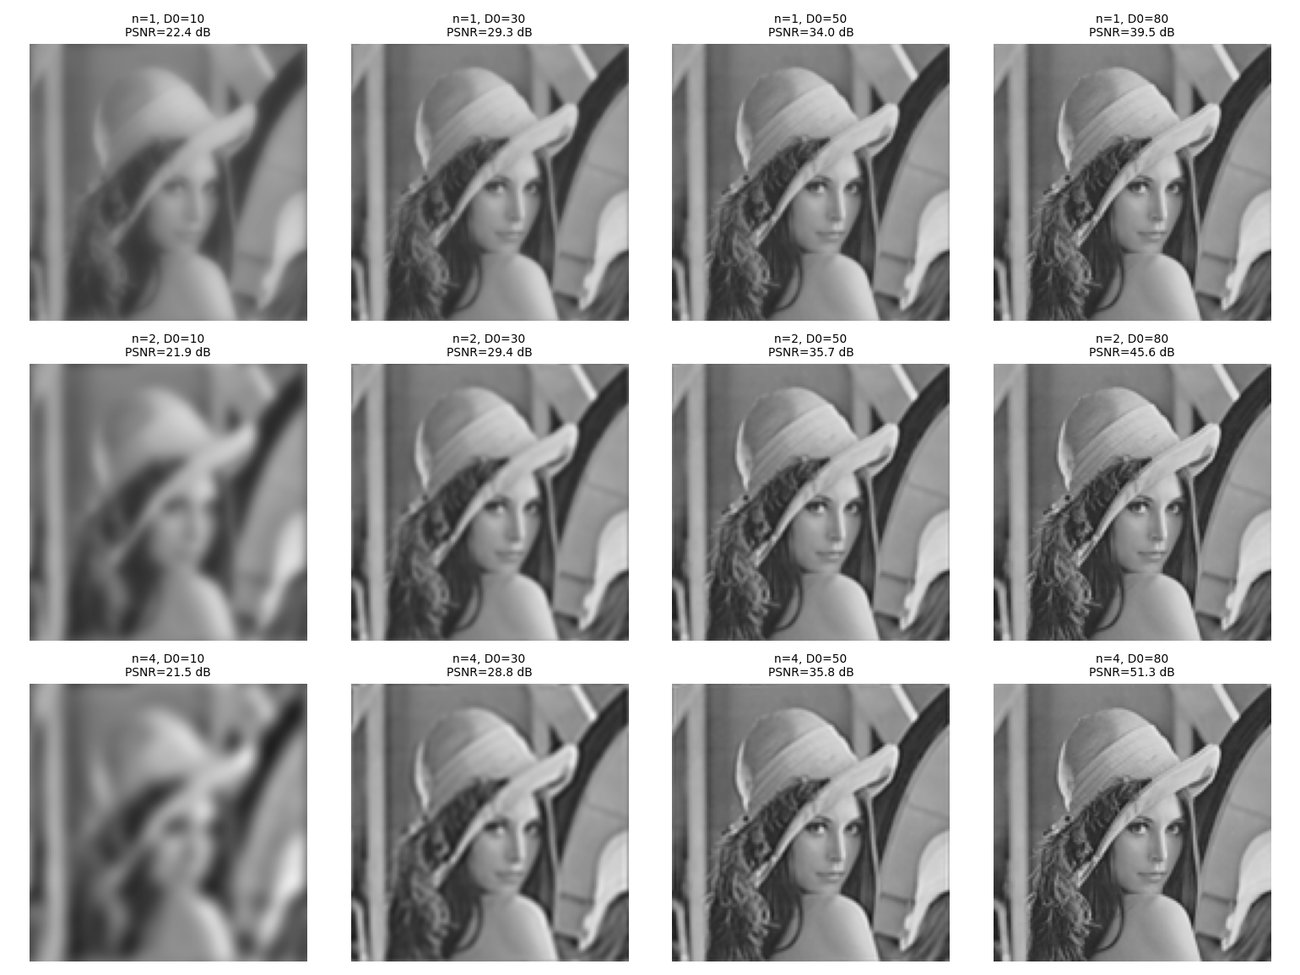
\includegraphics[width=0.9\textwidth]{bai4_butterworth_n_D0.jpg}
    \caption{Ảnh sau lọc Butterworth với $n=1,2,4$ (từng hàng) và $D_0=10,30,50,80$ (từng cột)}
\end{figure}

\begin{table}[H]
\centering
\begin{tabular}{lcccc}
\toprule
MSE & $D_0=10$ & $D_0=30$ & $D_0=50$ & $D_0=80$ \\
\midrule
$n=1$ & $374{,}7$ & $76{,}8$ & $26{,}0$ & $7{,}3$ \\
$n=2$ & $418{,}4$ & $75{,}2$ & $17{,}4$ & $1{,}8$ \\
$n=4$ & $460{,}3$ & $85{,}1$ & $17{,}1$ & $0{,}5$ \\
\bottomrule
\end{tabular}
\caption{MSE của bộ lọc Butterworth theo bậc $n$ và $D_0$}
\end{table}

\begin{figure}[H]
    \centering
    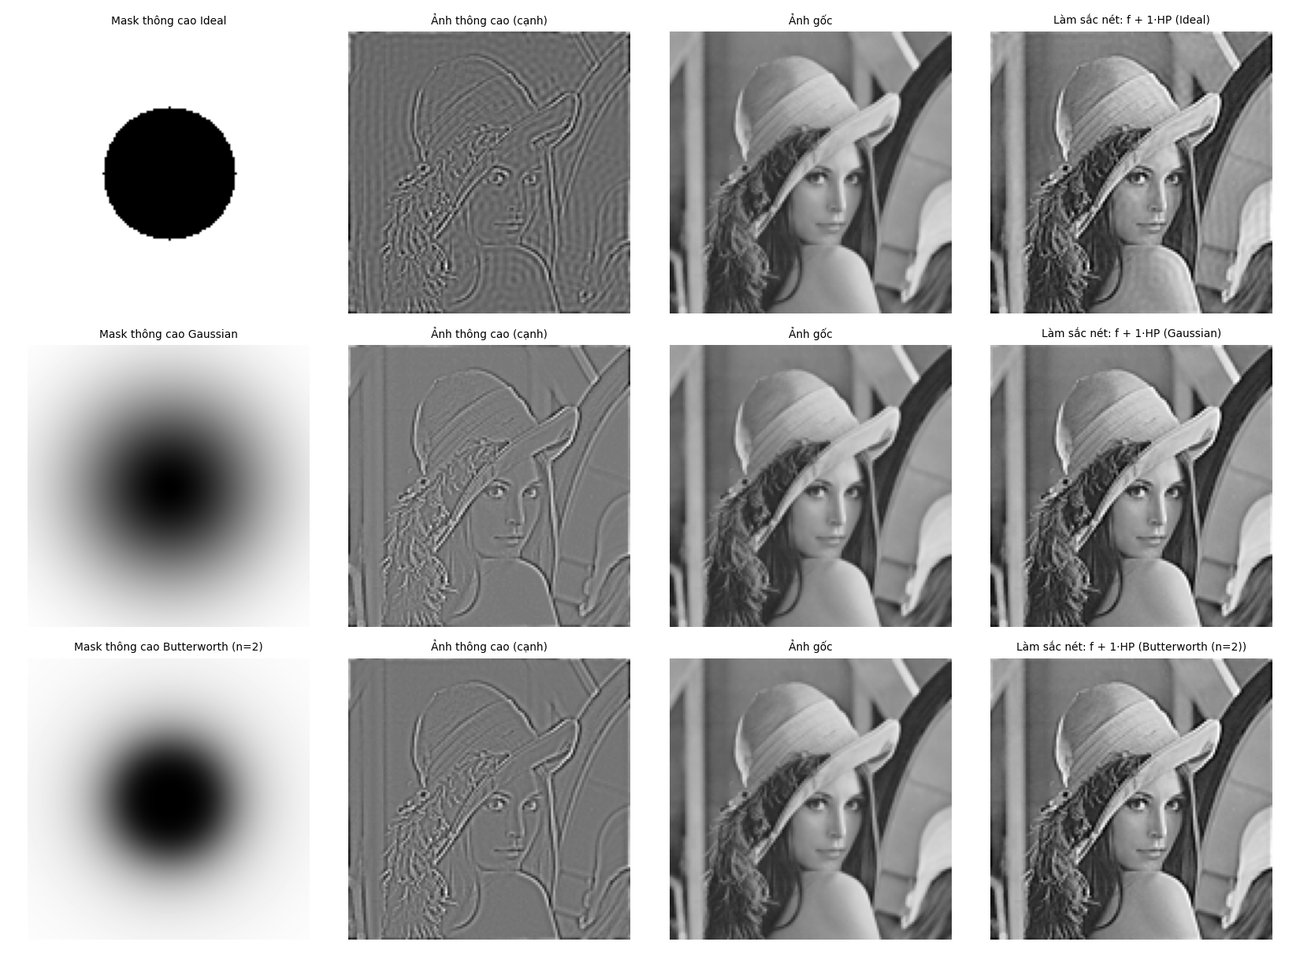
\includegraphics[width=0.9\textwidth]{bai4_thong_cao_sharpen.jpg}
    \caption{Mặt nạ thông cao, ảnh thông cao, ảnh gốc và ảnh làm sắc nét của ba bộ lọc ($D_0=30$)}
\end{figure}

\textbf{Nhận xét:}
\begin{itemize}
    \item Ở $D_0=30$, Ideal cho PSNR $27{,}9$ dB và có vân sóng quanh cạnh, Butterworth $n=2$ cho $29{,}4$ dB, Gaussian cho $30{,}6$ dB và mờ đều, không có vân sóng. Với $D_0=10,30,50$ thứ tự PSNR luôn là Gaussian, Butterworth, Ideal vì vân sóng của Ideal làm sai khác ảnh gốc ở nhiều pixel hơn.
    \item Với $D_0=80$ trên ảnh $128\times 128$, Ideal có PSNR cao nhất ($54{,}3$ dB) vì hình tròn đã chứa gần hết phổ, trong khi Gaussian vẫn làm suy giảm tần số cao ở mọi bán kính.
    \item Với $D_0$ nhỏ, $n$ lớn cho MSE lớn hơn vì bộ lọc cắt gắt hơn nên bỏ nhiều tần số ngay ngoài $D_0$. Với $D_0=80$ thì ngược lại, $n=4$ cho MSE nhỏ nhất ($0{,}5$) vì giữ gần nguyên các tần số bên trong $D_0$.
    \item Ảnh thông cao của Ideal có vân sóng lan trên vùng phẳng nên ảnh làm sắc nét có gợn sóng giả, còn Gaussian và Butterworth cho cạnh sạch và ảnh sắc nét hơn ảnh gốc.
\end{itemize}

Vì sao Ideal dễ gây ringing còn Gaussian chuyển tiếp mềm hơn? Bộ lọc Ideal có bước nhảy $0/1$ trong miền tần số, biến đổi ngược của nó là hàm sinc có các thuỳ dao động kéo dài, nên phép chập với sinc tạo vân sóng quanh cạnh mạnh. Biến đổi ngược của Gaussian vẫn là Gaussian, luôn dương và không dao động nên không có ringing.

Ảnh hưởng của bậc $n$ trong Butterworth là gì? Bậc $n$ điều khiển độ dốc quanh $D_0$: $n=1$ chuyển tiếp êm, gần Gaussian và không ringing nhưng lọc kém sắc, $n$ lớn tiệm cận Ideal, giữ tần số trong $D_0$ tốt hơn nhưng bắt đầu có ringing.Kết

%================ KẾT LUẬN ================
{\LARGE\bfseries Kết luận}\par\vspace{0.8em}
Bài thực hành đã cài đặt DFT, IDFT, DCT, IDCT bằng phép nhân ma trận mà không dùng hàm biến đổi có sẵn. DFT và IDFT khôi phục ảnh với sai số cỡ $10^{-24}$, DCT cho thấy năng lượng dồn vào hệ số DC và tần số thấp nên bỏ $50\%$ hệ số vẫn đạt PSNR khoảng $49{,}5$ dB. Khi lọc ảnh, Ideal gây ringing do bước nhảy đột ngột trong miền tần số, Gaussian cho kết quả mượt nhất, còn Butterworth nằm giữa và bậc $n$ điều chỉnh độ dốc của bộ lọc.

\vspace{1em}
Mã nguồn và kết quả thực nghiệm được đăng tại: \url{https://github.com/Maki1109/XLA_TH/tree/week4} (nhánh \texttt{week4}).

\end{document}
